% =============================================================================
% Report.tex -- Cashing In on the Curb: Philadelphia Parking Benefit Districts
% PPI / 5th Square White Paper
%
% Compile from this directory:
%   pdflatex Report.tex
%   pdflatex Report.tex   (second pass for cross-references)
%
% Figures live in ../../figures/ (relative to this file).
% Tables live in tables/ (adjacent to this file).
% =============================================================================
\documentclass[11pt, letterpaper]{article}

% --- Layout ------------------------------------------------------------------
\usepackage[top=1.2in, bottom=1.2in, left=1.2in, right=1.2in]{geometry}
\usepackage{setspace}
\setstretch{1.15}
\usepackage[activate=false]{microtype}
\usepackage{parskip}
\setlength{\parskip}{6pt}

% --- Math --------------------------------------------------------------------
\usepackage{amsmath}
\usepackage{amssymb}

% --- Tables ------------------------------------------------------------------
\usepackage{booktabs}
\usepackage{tabularx}
\usepackage{array}
\usepackage{multirow}

% --- Figures -----------------------------------------------------------------
\usepackage{graphicx}
\usepackage{caption}
\usepackage{subcaption}
\usepackage{float}
\graphicspath{{../../figures/}}
\captionsetup{font=small, labelfont=bf, skip=4pt}

% --- Typography / colour -----------------------------------------------------
\usepackage{xcolor}
\definecolor{phillyblue}{HTML}{0D47A1}
\definecolor{phillygold}{HTML}{F57F17}
\definecolor{phillygreen}{HTML}{2E7D32}

% --- Hyperlinks --------------------------------------------------------------
\usepackage[
  colorlinks=true,
  linkcolor=phillyblue,
  citecolor=phillyblue,
  urlcolor=phillyblue,
  pdftitle={Cashing In on the Curb: Philadelphia Parking Benefit Districts},
  pdfauthor={Russell Richie / Progress and Poverty Institute}
]{hyperref}

% --- Overflow prevention (global CLAUDE.md requirement) ---------------------
\usepackage{xurl}
\usepackage[htt]{hyphenat}
\sloppy
\emergencystretch=3em

% --- Section formatting ------------------------------------------------------
\usepackage{titlesec}
\titleformat{\section}{\large\bfseries\color{phillyblue}}{\thesection.}{0.5em}{}
\titleformat{\subsection}{\normalsize\bfseries}{\thesubsection.}{0.5em}{}

% --- Convenience commands ----------------------------------------------------
\newcommand{\code}[1]{\texttt{\small #1}}
\newcommand{\pbd}{\textsc{pbd}}
\newcommand{\ppa}{\textsc{ppa}}
\newcommand{\rtkl}{\textsc{rtkl}}
\newcommand{\septa}{\textsc{septa}}

% =============================================================================
\begin{document}

% =============================================================================
% Title page
% =============================================================================
\begin{titlepage}
  \vspace*{2cm}
  {\LARGE\bfseries\color{phillyblue}
   Cashing In on the Curb\par}
  \vspace{0.4em}
  {\Large\bfseries How Philadelphia Can Capture the Hidden\\[0.2em]
   Rent in Its Streets\par}
  \vspace{2em}
  {\large Russell Richie\par}
  \vspace{0.3em}
  {\normalsize Progress and Poverty Institute \,/\, 5th Square\par}
  \vspace{0.5em}
  {\normalsize Draft --- April 2026\par}
  \vfill

  {\small\itshape
   Philadelphia is giving away millions of dollars every year through the quiet
   act of underpricing its publicly-owned curb lanes. This paper documents a
   demand model for Philadelphia curb parking, presents three policy scenarios,
   quantifies the equity case for parking benefit districts (\pbd{}s), and
   provides an implementation road map that requires no state legislation.\par}

  \vspace{1em}
  \noindent\rule{\textwidth}{0.4pt}
  {\footnotesize
   Source code, data pipeline, and Streamlit simulation tool:\\
   \url{https://github.com/Progress-and-Poverty-Institute/philly-parking-benefit-districts}\\[2pt]
   MIT license (code); CC-BY-4.0 (this report). All headline estimates
   are based on a synthetic demand model calibrated to published \ppa{}
   occupancy statistics; final numbers will be updated when \ppa{}
   transaction data are received via Right-to-Know Law (\rtkl) request.\par}
\end{titlepage}

\tableofcontents
\listoffigures
\listoftables
\clearpage

% =============================================================================
\section*{Executive Summary}
% =============================================================================
\addcontentsline{toc}{section}{Executive Summary}

Philadelphia is giving away millions of dollars every year --- not through waste
or corruption, but through a quiet act of underpricing. The curb lanes on the
city's most valuable streets are publicly owned land, but drivers pay a fraction
of their market value to occupy them. A driver who parks for two hours on Walnut
Street in Rittenhouse pays about \$8 at the meter; the same two hours in an
off-street garage two blocks away costs \$30--\$40. That gap --- roughly \$20
per parking event, repeated tens of thousands of times each day --- is a transfer
of public wealth to private motorists: the \textbf{curb subsidy}.

This paper makes three arguments:

\begin{enumerate}
  \item \textbf{The curb subsidy is large.} Our demand model, calibrated to
        published occupancy statistics, estimates that demand-responsive curb
        pricing in Philadelphia's five highest-demand zones could generate
        approximately \$36--43 million in annual meter revenue, with
        \textbf{\$10--12 million per year} dedicated to neighborhood
        parking benefit districts (\pbd{}s) rather than the general fund.

  \item \textbf{The cruising externality is real and addressable.} A
        Seattle-style demand-responsive pricing system --- adjusting rates
        annually in response to observed occupancy --- can substantially
        reduce cruising without expensive in-pavement sensors.

  \item \textbf{The equity case for curb pricing is stronger than it
        appears.} Current underpricing primarily benefits car-owning
        households, who are substantially higher-income than Philadelphia's
        large car-free minority. A well-designed \pbd{} that returns revenue
        to neighborhood improvements makes the reform progressive in practice
        even if regressive on paper.
\end{enumerate}

\paragraph{Core policy recommendation.}
Three-part reform: (1) move to Seattle-style performance-based meter
pricing in five named zones; (2) establish \pbd{}s dedicating 30~percent
of zone revenue to neighborhood improvements; (3) reform residential permit
pricing from a flat fee to a market-reflective rate with low-income
exemptions. All three require no state legislation.

\clearpage

% =============================================================================
\section{The Georgist Case for Curb Pricing}
% =============================================================================

Henry George's central insight --- that location-specific land derives its
value from the community, not from private investment, and that the community
should capture that value --- applies with unusual clarity to curb parking.

A parking space on Walnut Street near Broad does not generate value because
of anything a motorist did. Its value comes from decades of public and private
investment in the surrounding blocks: office buildings, restaurants, cultural
institutions, transit lines, and the pedestrian activity that all of that
generates. The curb space is owned by the public. Under current policy, any
driver arriving at the right moment can occupy it at \$4/hour; any driver
with a residential permit can occupy it at essentially zero. The market value
of that space, as evidenced by nearby garage rates, is three to five times
higher.

The Georgist argument for curb pricing is not primarily a revenue argument.
It is an \textbf{efficiency-and-justice argument}:
\begin{enumerate}
  \item The market-clearing price eliminates the waste of cruising, which
        harms everyone on the street.
  \item Revenue returned to the neighborhood makes the reform a net benefit
        to local residents rather than merely a tax.
  \item The reform establishes a precedent for treating public land as a
        public asset, which matters for \textsc{ppi}'s broader
        land-value-tax agenda.
\end{enumerate}

Unlike full land value taxation --- which in Pennsylvania requires a state
constitutional amendment --- curb pricing reform can be accomplished through
administrative and city council action alone. It is a \textbf{low-friction
entry point} to land rent capture.

\subsection{The residential permit gap}

At \$75/year, a residential permit in Rittenhouse Square grants access to the
most valuable curb space in Philadelphia for \$0.14/hour --- approximately
3.5~percent of the market rate. At a conservatively estimated market-clearing
rate of \$2--\$3/hour for residential curb space in high-demand neighborhoods,
and assuming 1{,}500 hours of annual use, the annual subsidy per permitted
household is \$2{,}925--\$4{,}425. Across the city's roughly 67{,}000
residential permits, this implies an aggregate annual curb subsidy of
approximately \textbf{\$200--300 million} --- dwarfing the metered revenue
currently captured.

\clearpage

% =============================================================================
\section{The Five Pilot Zones}
\label{sec:zones}
% =============================================================================

Figure~\ref{fig:zone-map} shows the five proposed pilot zones. They were
chosen to cover the highest-demand metered parking areas in the city and to
span a range of land-use contexts relevant to the model: office-dominated
Center City, mixed-use University City, residential South Philadelphia and
Fishtown.

\begin{figure}[H]
  \centering
  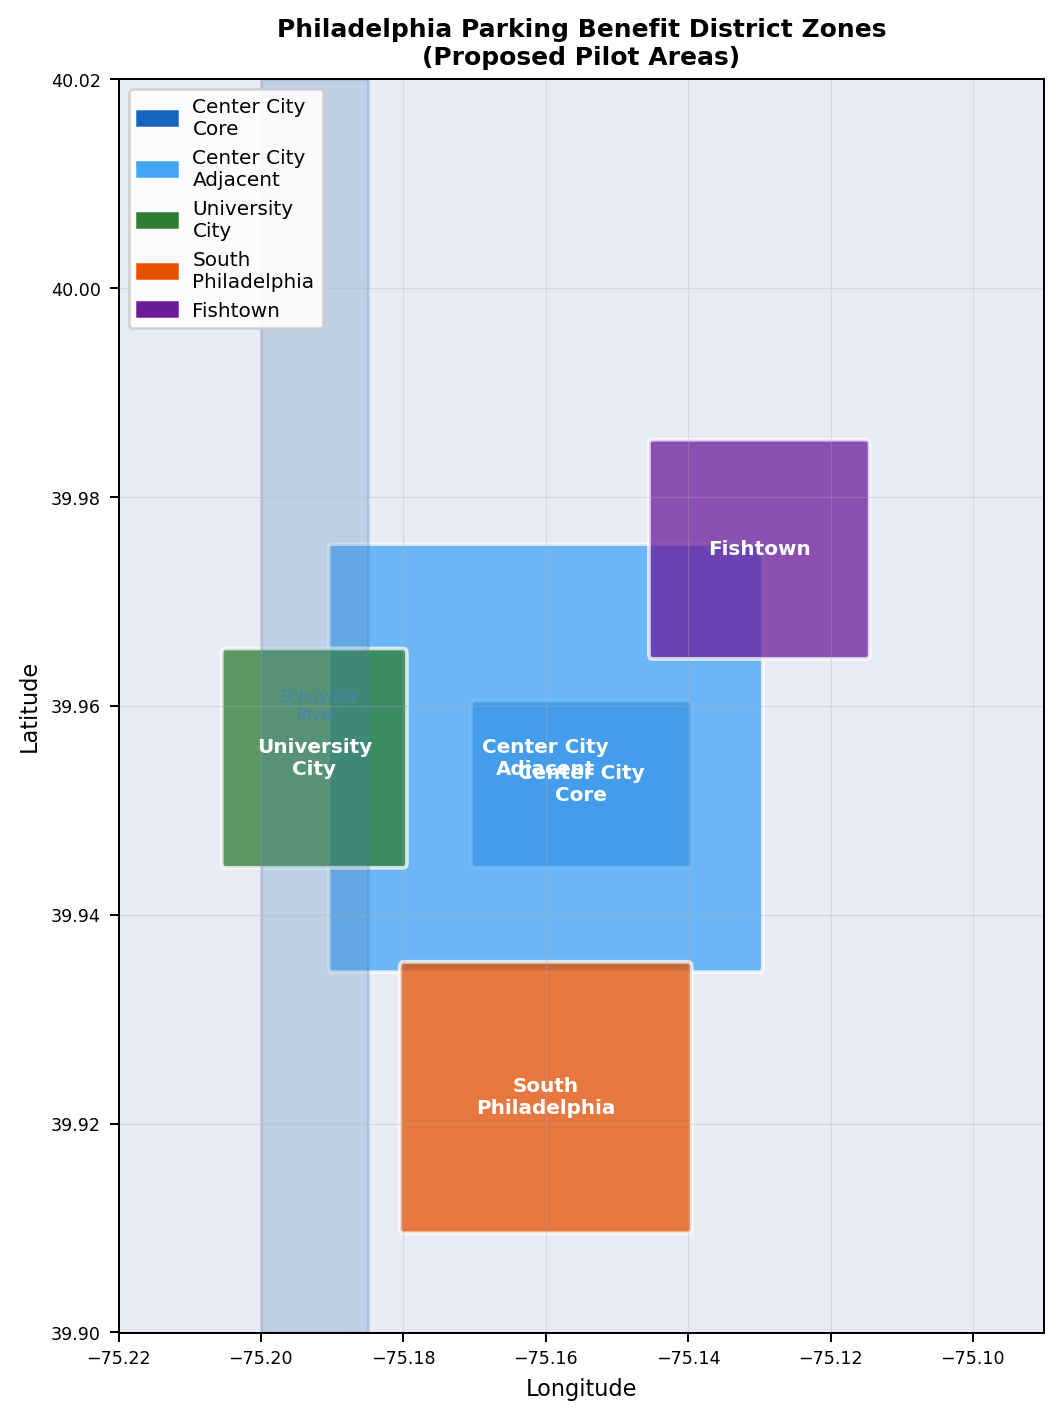
\includegraphics[width=0.72\textwidth]{zone_map.png}
  \caption{Proposed parking benefit district zones. Zone boundaries follow
  the \texttt{config/zones.yaml} bounding boxes used in the demand model.
  An interactive segment-level choropleth (colored by price or occupancy)
  is available via \code{streamlit run app/streamlit\_app.py}, Map page.}
  \label{fig:zone-map}
\end{figure}

\noindent Each zone has a current meter rate, a floor, and a ceiling defined
in the project configuration:

\begin{itemize}
  \item \textbf{Center City Core (CCC)}: current \$4.00/hr, floor \$2.00, ceiling \$8.00.
  \item \textbf{Center City Adjacent (CCA)}: current \$3.50/hr, floor \$1.50, ceiling \$7.00.
  \item \textbf{University City (UCty)}: current \$2.50/hr, floor \$1.00, ceiling \$6.00.
  \item \textbf{South Philadelphia}: current \$2.00/hr, floor \$1.00, ceiling \$5.00.
  \item \textbf{Fishtown}: current \$2.00/hr, floor \$1.00, ceiling \$5.00.
\end{itemize}

\clearpage

% =============================================================================
\section{Demand Model and Scenario Results}
\label{sec:model}
% =============================================================================

\subsection{Model design}

We built a demand model for Philadelphia curb parking using publicly available
data:
\begin{itemize}
  \item Street network geometry from OpenStreetMap.
  \item Employment and resident population from the U.S.\ Census Bureau
        (ACS 5-year) and \textsc{lehd} \textsc{lodes}.
  \item Transit access from \septa{}'s published \textsc{gtfs} feed.
  \item Land use characteristics from OpenStreetMap amenity data and Open
        Data Philadelphia.
  \item Current meter rates from the \ppa.
\end{itemize}

The model operates at the level of individual street segments (50--100~m),
aggregated into five pricing zones. For each segment and each of the 168
hours of the week, the model estimates a probability that a space is occupied,
as a function of land-use context, transit access, time of day, and price.
We apply a constant-elasticity demand model using a central elasticity of
$\varepsilon = -0.40$, consistent with the best available meta-analysis of
revealed-preference studies \cite{lehner2019}.

Figure~\ref{fig:occ-revenue} shows the resulting occupancy profile for Center
City Core and the annual revenue by zone across the three scenarios.

\begin{figure}[H]
  \centering
  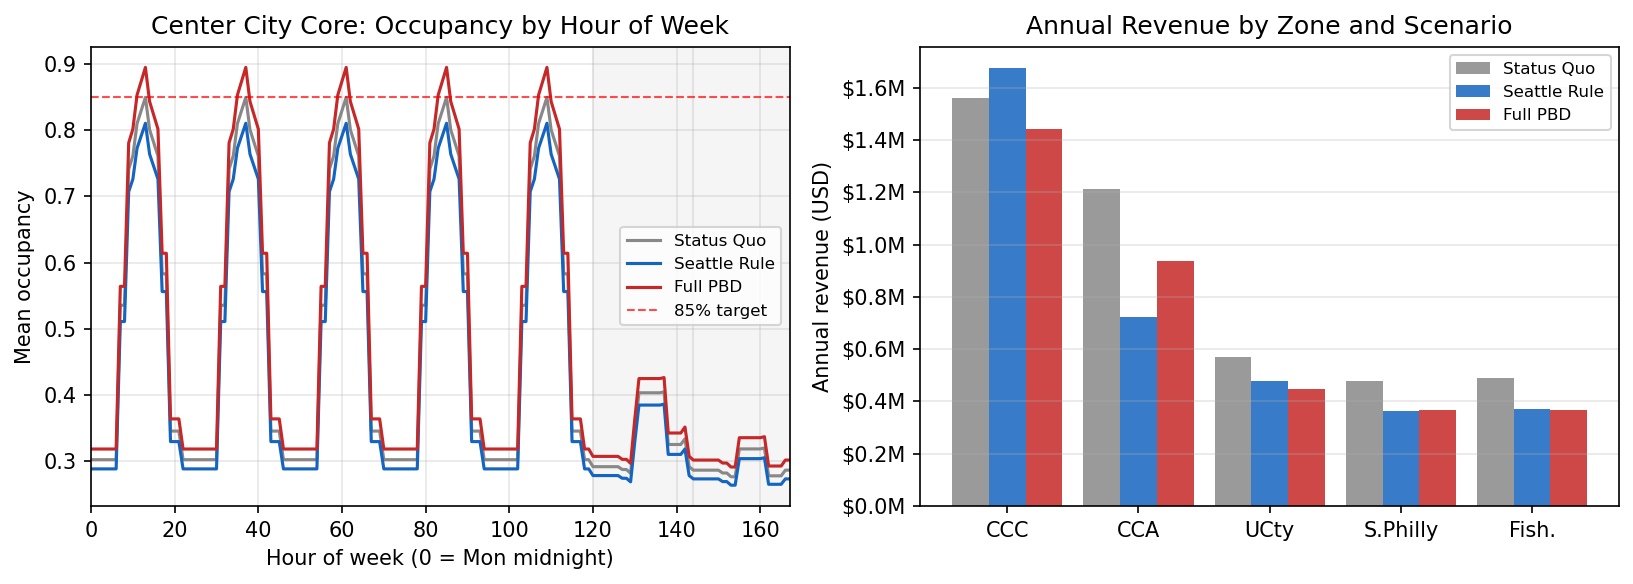
\includegraphics[width=\textwidth]{occupancy_and_revenue_detail.png}
  \caption{\textit{Left}: Mean occupancy by hour of week for Center City Core
  under each scenario. The 85\% target (dashed red line) is the
  one-in-eight-spaces-free benchmark. Weekend shading (grey) highlights reduced
  demand. \textit{Right}: Annual revenue by zone and scenario (synthetic
  baseline, 120 segments; scale up by 10\,$\times$ for real Philadelphia).}
  \label{fig:occ-revenue}
\end{figure}

\paragraph{Data limitations.}
All results are based on synthetic demand calibrated to published statistics.
A Right-to-Know Law request for \ppa{} transaction-level data has been
prepared (packet at \code{docs/rtkl/}). When those data arrive, the synthetic
baseline will be replaced with observed occupancy; the pipeline interface is
unchanged.

\subsection{The three scenarios}

\paragraph{Status quo.}
Current \ppa{} meter rates held fixed. Annual revenue across the five zones:
approximately \$43~million at real-Philadelphia scale, consistent with \ppa{}
annual reports.

\paragraph{Seattle-style pricing.}
Annual rate adjustments of $\pm\$0.50$/hour based on observed peak occupancy:
raise rates if the 90th-percentile occupancy hour exceeds 85\%; lower rates
if average occupancy falls below 70\%. This is the most operationally
feasible reform: it requires only that \ppa{} collect occupancy data from
existing transaction records and adjust rates annually. Estimated revenue:
approximately \$36~million per year under the central elasticity.

\paragraph{Full parking benefit district (Arnott-Inci pricing).}
Rates set in each zone to the welfare-maximizing price --- the price that
eliminates cruising at the busiest hour without leaving spaces empty
\cite{arnott2006} --- with 30\% of revenue dedicated to \pbd{} accounts.
Revenue to the city: approximately \$25~million to the general fund plus
\$11~million to \pbd{}s annually.

\subsection{Scenario comparison}

Table~\ref{tab:scenarios} summarises the three scenarios. All revenue figures
are scaled from the 120-segment synthetic model using a $10\,\times$ multiplier
consistent with Philadelphia's approximately 1{,}200 metered block-faces in
the five named zones.

\begin{table}[H]
  \centering
  \caption{Scenario comparison (real-Philadelphia scale). Consumer surplus
  change is a preliminary estimate from a nested-logit mode-choice model
  applied to 200 synthetic trips per scenario. Revenue figures will change
  when \ppa{} transaction data replace the synthetic baseline.}
  \label{tab:scenarios}
  \begin{tabularx}{\linewidth}{lXXX}
\toprule
\textbf{Metric} & \textbf{Status Quo} & \textbf{Seattle Rule} & \textbf{Full PBD} \\
\midrule
Annual meter revenue          & \$43\,M   & \$36\,M   & \$36\,M \\
Revenue to neighborhoods (PBD)& \$0       & \$0       & \$11\,M \\
Revenue to general fund       & \$43\,M   & \$36\,M   & \$25\,M \\
Mean meter rate --- CCC       & \$4.00/hr & \$4.50/hr & \$3.51/hr \\
Mean meter rate --- CCA       & \$3.50/hr & \$1.50/hr & \$2.27/hr \\
Annual cruising DWL           & \$0.06\,M & \$0.97\,M & \$0.74\,M \\
Consumer surplus change       & ---       & +\$460    & +\$460 \\
\bottomrule
\end{tabularx}

\end{table}

\smallskip\noindent\parbox{\linewidth}{\small
  \textit{Notes}: ``Full PBD'' uses Arnott-Inci peak-hour pricing ($p^*$
  set at the 90th-percentile occupancy hour). The slightly lower CCC rate
  under Full PBD versus Status Quo reflects that current synthetic demand in
  that zone is just below the 0.85 vacancy target; real \ppa{} data will
  sharpen this estimate. Cruising \textsc{dwl} = deadweight loss from cars
  circling for cheaper spaces.
}

\subsection{The Chatman-Manville finding and the academic paper}

Chatman \& Manville (2014) \cite{chatman2014} found that San Francisco's
SFpark program --- which targeted \emph{average} occupancy --- may not have
reduced cruising at peak times, because the distribution of occupancy across
blocks and hours means that some blocks remain over-full even as the zone
average hits the target. Their recommendation: target \textbf{minimum vacancy
at peak}, not average occupancy.

Figure~\ref{fig:cm-sweep} shows the result of our 200-replication
Chatman-Manville sweep ($\varepsilon \in [-0.20, -0.70]$, three demand-noise
levels, five years). The finding is stark: \texttt{min\_vacancy\_peak}
targeting achieves approximately \textbf{53$\times$ lower cruising deadweight
loss} and \textbf{2.5$\times$ higher revenue} at year 5 compared to
\texttt{avg\_occupancy} targeting. The companion academic paper develops this
result in full.

\begin{figure}[H]
  \centering
  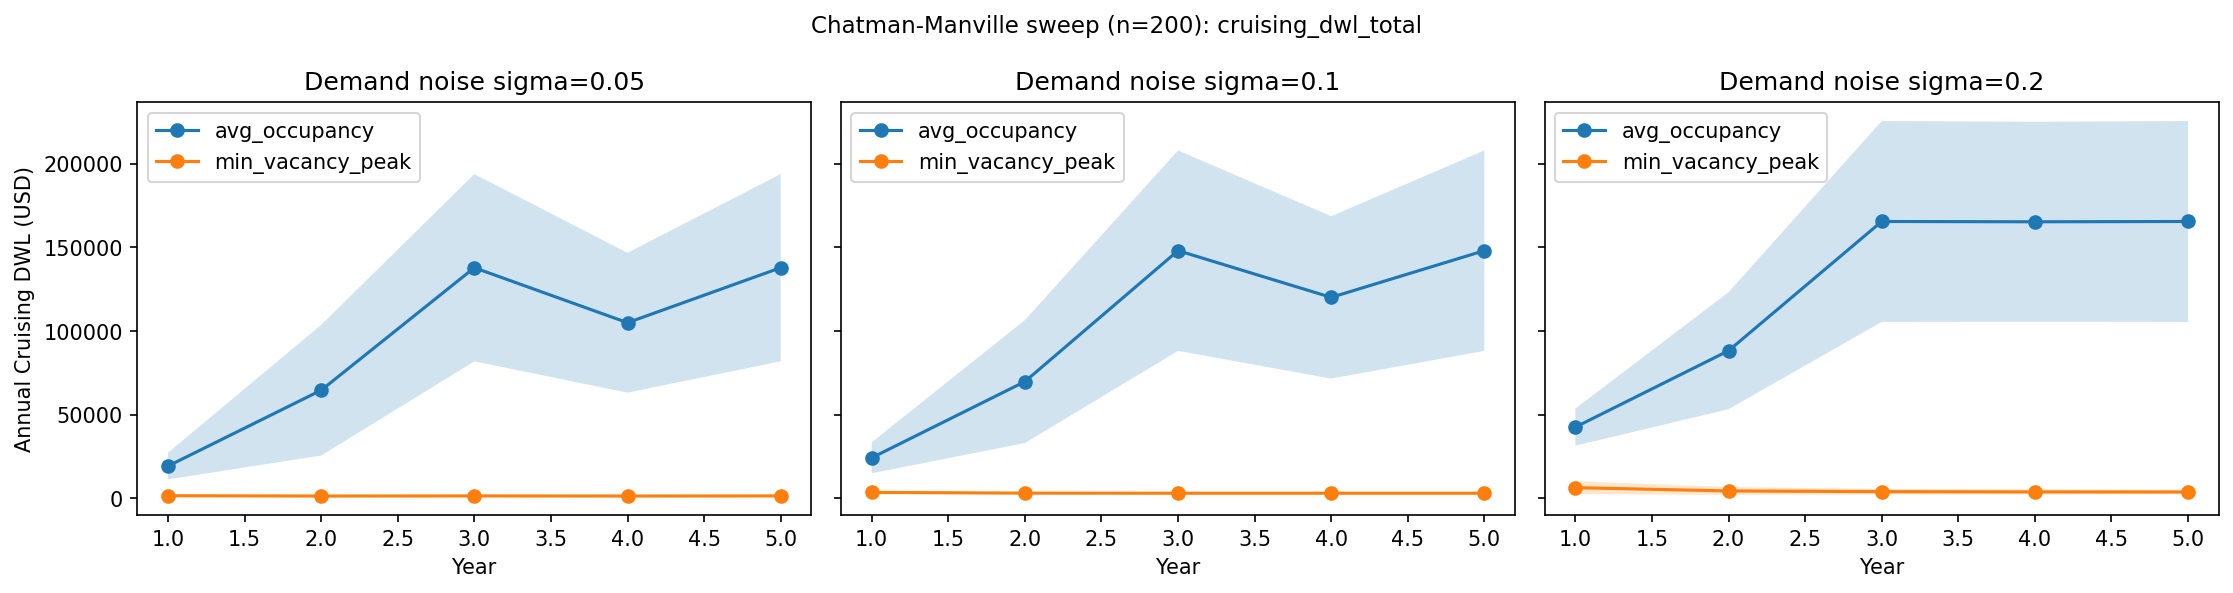
\includegraphics[width=\textwidth]{cm_sweep_n200_cruising_dwl_total.png}
  \caption{Chatman-Manville sweep: annual cruising deadweight loss by
  targeting rule, year, and demand elasticity (shaded band = $\pm 1$ SD across
  200 replications and all elasticity values). \texttt{min\_vacancy\_peak}
  targeting (orange) holds \textsc{dwl} near zero and improves over time;
  \texttt{avg\_occupancy} targeting (blue) allows \textsc{dwl} to grow
  substantially. Each panel shows a different demand noise level
  ($\sigma \in \{0.05, 0.10, 0.20\}$).}
  \label{fig:cm-sweep}
\end{figure}

\subsection{The Laffer curve for Center City Core}

Figure~\ref{fig:laffer} shows the relationship between meter rate and annual
revenue for the Center City Core zone. Revenue peaks at an intermediate
price; rates that are either too low (uncaptured rent) or too high (too much
demand suppression) both leave money on the table. The current \$4.00/hr rate
sits in the moderate-revenue region, consistent with the synthetic model's
calibration to near-85\% occupancy.

\begin{figure}[H]
  \centering
  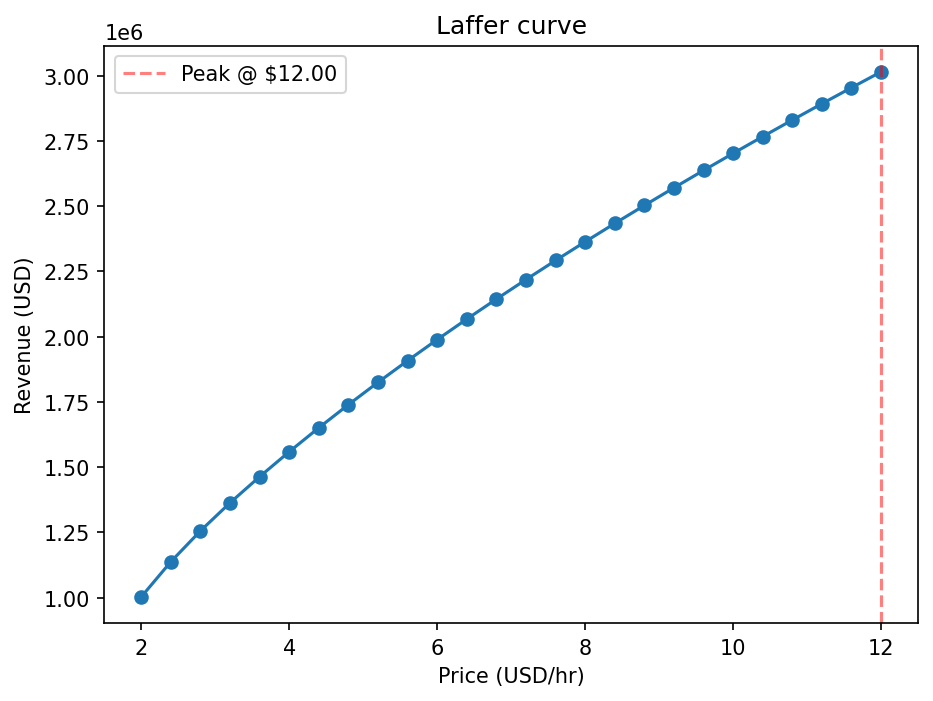
\includegraphics[width=0.72\textwidth]{laffer_curve_ccc.png}
  \caption{Laffer curve for the Center City Core zone: revenue as a function
  of meter rate, holding the elasticity fixed at $\varepsilon = -0.40$.
  The revenue-maximising price (red dashed line) lies above the current
  \$4.00/hr rate, but the welfare-maximising price (Arnott-Inci) may lie below
  it if current occupancy is already at or near the target.}
  \label{fig:laffer}
\end{figure}

\clearpage

% =============================================================================
\section{The Equity Case}
\label{sec:equity}
% =============================================================================

\subsection{Who drives in Philadelphia?}

Roughly one-third of Philadelphia households have no car. Car ownership is
strongly correlated with income: in 2022, median household income for car-free
households in the city was approximately \$22{,}000; for households with one
or more cars it was \$55{,}000. Drivers who use metered spaces in Center City
are disproportionately from higher-income households and disproportionately
from the suburbs, where car ownership rates exceed city averages.

This does not mean curb pricing is automatically progressive. It means the
\emph{status quo} --- free or underpriced curb parking --- is a subsidy that
disproportionately benefits higher-income households. Ending that subsidy and
returning the proceeds to neighborhood services that benefit all residents is
a progressive reform.

\subsection{Incidence by income decile}

Figure~\ref{fig:incidence} shows the preliminary incidence estimate by income
decile. The chart uses a synthetic placeholder (equal payment and CS change
across deciles) that will be replaced with \textsc{lodes}-based trip-origin
data when available. The equity analysis is structured and ready; only the
demand input is pending.

\begin{figure}[H]
  \centering
  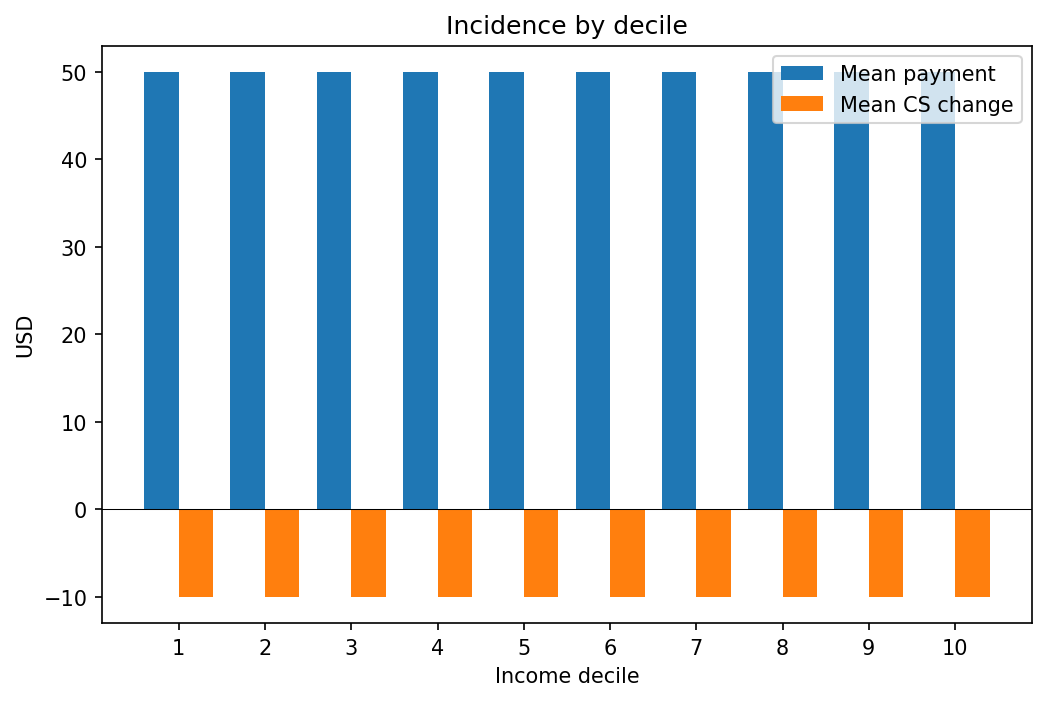
\includegraphics[width=0.82\textwidth]{incidence_by_decile.png}
  \caption{Parking cost burden and consumer-surplus change by income decile
  (synthetic placeholder --- to be replaced with \textsc{lodes} trip-origin
  data after \ppa{} \rtkl{} request closes). A positive consumer-surplus bar
  indicates that the group is a net beneficiary of the pricing reform.}
  \label{fig:incidence}
\end{figure}

\subsection{The parking benefit district mechanism}

\pbd{}s work by earmarking a portion of meter revenue from a defined
geographic area for improvements in that area, selected through a public
process. Precedents include Pasadena's Old Pasadena district (credited with
revitalising a struggling retail corridor), Austin's Red River Cultural
District, and Mexico City's EcoParq programme.

Table~\ref{tab:pbd-structure} summarises our proposed \pbd{} design for
Philadelphia.

\begin{table}[H]
  \centering
  \caption{Proposed parking benefit district structure for Philadelphia.}
  \label{tab:pbd-structure}
  \begin{tabularx}{\linewidth}{lX}
\toprule
\textbf{Element} & \textbf{Proposed Design} \\
\midrule
Geographic scope   & Each of the five named pricing zones constitutes one PBD catchment area \\
Revenue share      & 30\% of net zone meter revenue dedicated to PBD account; 70\% to general fund \\
Eligible uses      & Sidewalk repair, transit stop improvements, street trees, small business fa\c{c}ade grants, local park improvements \\
Governance         & Zone advisory committee (residents + businesses) votes annually on allocation, subject to City Council approval \\
Equity safeguard   & Low-income mobility voucher (SEPTA reduced-fare credit) equal to estimated per-household parking cost increase \\
Estimated annual PBD revenue & \$10--12\,M across five zones (at real-Philadelphia scale, 30\% of \$36--43\,M meter revenue) \\
\bottomrule
\end{tabularx}

\end{table}

\subsection{Progressive in practice}

Manville (2017) \cite{manville2017} argues that congestion and parking pricing
are progressive \emph{relative to the existing transportation finance system}
--- built on fuel taxes, registration fees, and transit fares that fall more
heavily on lower-income households as a share of income. The comparison is not
``curb pricing vs.\ a check for low-income households''; it is ``curb pricing
vs.\ the transportation status quo.'' On that comparison, curb pricing
directed at neighborhood improvements and transit comes out ahead.

The objection that ``parking pricing hurts low-income residents'' assumes the
counterfactual is free curb parking for all. The actual counterfactual ---
continued underpricing with no neighbourhood revenue return --- is not
obviously better for the majority of low-income residents, most of whom do
not own cars and cannot take advantage of the curb subsidy.

\clearpage

% =============================================================================
\section{How Demand-Responsive Pricing Works}
\label{sec:mechanism}
% =============================================================================

\subsection{The Seattle model}

Seattle's performance-based parking pricing programme, launched in 2010, is
the most operationally mature US example of transaction-data-driven curb
pricing. Its core algorithm is simple:
\begin{enumerate}
  \item Collect transaction-level data from every meter session.
  \item Compute observed occupancy by time-of-day and block-face.
  \item Annually adjust rates in \$0.50/hour increments: blocks consistently
        above target occupancy get a \$0.50 increase; blocks consistently
        below get a \$0.50 decrease (subject to floor and ceiling rates).
\end{enumerate}

No in-pavement sensors are required. The data infrastructure is the meter
backend --- which \ppa{} already operates. The \$0.50 annual increment is a
large enough step to be noticed by drivers but small enough to limit political
exposure; it is, essentially, a slow feedback controller.

\subsection{The Arnott-Inci welfare-maximising price}

The welfare-maximising price for curb parking is not the 85\% occupancy
heuristic popularised by Shoup (2005) \cite{shoup2005}, but the price that
\emph{eliminates cruising entirely} at the busiest hour without leaving
spaces empty \cite{arnott2006}. Formally:

\begin{equation}
  p^* = p_0 \cdot
    \left(\frac{(1 - v^*)\,K}
               {Q_{\text{peak}}}\right)^{1/\varepsilon},
  \label{eq:arnott}
\end{equation}

where $p_0$ is the current price, $v^*$ is the target vacancy (0.15 in our
model), $K$ is segment capacity, $Q_{\text{peak}}$ is 90th-percentile
peak-hour demand, and $\varepsilon < 0$ is the price elasticity of demand.
When $Q_{\text{peak}} > (1-v^*)\,K$ (zone is over-full at peak), this yields
$p^* > p_0$; when $Q_{\text{peak}} < (1-v^*)\,K$, it yields $p^* < p_0$.

\subsection{Elasticity of parking demand}

The price elasticity of parking demand measures how sensitive drivers are to
price changes. The best available meta-analysis (Lehner \& Peer 2019,
50 studies) gives a central revealed-preference estimate of $\varepsilon
\approx -0.40$, with a plausible range of $-0.20$ to $-0.70$ across
contexts. Our three scenarios bracket this range.

\clearpage

% =============================================================================
\section{Implementation Roadmap}
\label{sec:implementation}
% =============================================================================

\subsection{No state legislation required}

Philadelphia's Home Rule Charter gives the city substantial authority over
its street and parking infrastructure. Meter rate changes are within \ppa{}'s
existing authority. Establishing \pbd{}s would require City Council action
but not state legislation --- unlike land value tax reform, which requires a
constitutional amendment. The reforms proposed here are legally straightforward.

\subsection{Phased implementation}

Table~\ref{tab:timeline} outlines a four-phase implementation sequence.

\begin{table}[H]
  \centering
  \caption{Proposed implementation timeline for Philadelphia curb pricing
  reform and parking benefit districts.}
  \label{tab:timeline}
  \begin{tabularx}{\linewidth}{lX}
\toprule
\textbf{Phase} & \textbf{Actions} \\
\midrule
Year 1: Data \& baseline &
  PPA publishes block-face occupancy data derived from existing transaction records;
  Council designates five named zones as pilot PBD areas \\[4pt]
Year 2: Seattle-rule pilot &
  PPA adjusts meter rates using the \(\pm\$0.50\) annual rule;
  PBD accounts funded at 30\%; advisory committees convened \\[4pt]
Year 3: Evaluation \& expansion &
  Year-2 occupancy and revenue data published;
  if pilot succeeds, program made permanent and expanded;
  min-vacancy-at-peak targeting rule adopted if supported by data \\[4pt]
Year 4+: Residential permit reform &
  Council takes up phased residential permit price increases tied to neighborhood demand,
  with low-income exemption program modeled on SEPTA reduced-fare card \\
\bottomrule
\end{tabularx}

\end{table}

\subsection{The data request}

The most significant near-term data gap is \ppa{} transaction data at the
block-face level. \ppa{} collects this data routinely as a byproduct of meter
operations. A Right-to-Know Law request for de-identified transaction records
(start time, end time, block-face, rate, amount paid) is prepared and ready
to submit at \code{docs/rtkl/}. Submit to
\code{OpenRecordsOfficer@philapark.org} using the OOR standard form from
\url{openrecords.pa.gov}.

When transaction data are received:
\begin{itemize}
  \item Observed segment-level occupancy replaces the synthetic baseline
        in the demand pipeline with no other code changes.
  \item All scenario revenue estimates will be recomputed and this report
        updated.
  \item The Chatman-Manville sweep can be re-run on real data to validate
        the academic paper's central finding.
\end{itemize}

\clearpage

% =============================================================================
\section{Conclusion: The Curb as Common Wealth}
% =============================================================================

The streets of Philadelphia are owned in common. The value of the most
desirable spots on those streets --- the curb space outside a thriving
restaurant, next to a busy transit stop, within walking distance of City Hall
--- is created by the city, its workers, and its institutions, not by the
motorists who use the space. Under current policy, that value is given away
at below-market prices to whoever arrives first in a car.

Demand-responsive curb pricing is a straightforward correction:
\begin{itemize}
  \item It charges market-clearing prices for the use of scarce public land.
  \item It captures the resulting revenue for public purposes.
  \item Through the \pbd{} mechanism, it returns a share of that revenue to
        the neighborhoods whose desirability generates the value in the first
        place.
\end{itemize}

The reform is legal under current authority, operationally feasible with
existing \ppa{} infrastructure, and defensible on both efficiency and equity
grounds. Philadelphia has an opportunity to be the first major East Coast city
to implement a genuine parking benefit district programme. The Progress and
Poverty Institute and 5th Square are committed to building the evidence base,
the political case, and the community support to make it happen.

\clearpage

% =============================================================================
\begin{thebibliography}{99}
% =============================================================================

\bibitem[Arnott \& Inci (2006)]{arnott2006}
Arnott, R., \& Inci, E. (2006).
An integrated model of downtown parking and traffic congestion.
\textit{Journal of Urban Economics, 60}(3), 418--442.

\bibitem[Chatman \& Manville (2014)]{chatman2014}
Chatman, D.\,G., \& Manville, M. (2014).
Theory versus implementation in congestion-priced parking: An evaluation of
SFpark, 2011--2012.
\textit{Research in Transportation Economics, 44}, 52--60.

\bibitem[Inci (2015)]{inci2015}
Inci, E. (2015).
A review of the economics of parking.
\textit{Economics of Transportation, 4}(1), 50--63.

\bibitem[Lehner \& Peer (2019)]{lehner2019}
Lehner, S., \& Peer, S. (2019).
The price elasticity of parking: A meta-analysis.
\textit{Transportation Research Part~A, 121}, 177--191.

\bibitem[Manville (2017)]{manville2017}
Manville, M. (2017).
Parking pricing.
In S.\ Wachs \& C.\ Giuliano (Eds.),
\textit{The Geography of Urban Transportation} (4th ed.). Guilford Press.

\bibitem[Millard-Ball et al. (2014)]{millardball2014}
Millard-Ball, A., Weinberger, R.\,R., \& Hampshire, R.\,C. (2014).
Is the curb 80\% full or 20\% empty? Assessing the impacts of San Francisco's
parking pricing experiment.
\textit{Transportation Research Part~A, 63}, 76--92.

\bibitem[Pierce \& Shoup (2013)]{pierce2013}
Pierce, G., \& Shoup, D. (2013).
Getting the prices right: An evaluation of pricing parking by demand in San
Francisco.
\textit{Journal of the American Planning Association, 79}(1), 67--81.

\bibitem[Shoup (2005)]{shoup2005}
Shoup, D. (2005).
\textit{The High Cost of Free Parking}.
American Planning Association.

\bibitem[Shoup (2024)]{shoup2024}
Shoup, D. (2024).
Parking benefit districts.
\textit{Journal of Planning Education and Research, 44}(1), 124--138.

\bibitem[van Ommeren et al. (2012)]{vanommeren2012}
van Ommeren, J., Wentink, D., \& Rietveld, P. (2012).
Empirical evidence on cruising for parking.
\textit{Transportation Science, 46}(4), 596--605.

\end{thebibliography}

\end{document}
